\documentclass[10pt,red]{beamer} 
% change the alerted colour to blue
\setbeamercolor{alerted text}{fg=blue}

\usetheme{berlin}
% theme split
\usepackage{beamerthemesplit}

\usepackage{booktabs,array,}
\usepackage{listings}
\usepackage{hyperref}
\usepackage{verbatim,moreverb}
\usepackage{tikz}

\usepackage{color}

\definecolor{dkgreen}{rgb}{0,0.6,0}
\definecolor{gray}{rgb}{0.5,0.5,0.5}
\definecolor{mauve}{rgb}{0.58,0,0.82}

\lstset{frame=tb,
  language = Java,
  aboveskip=3mm,
  belowskip=3mm,
  showstringspaces=true,
  columns=flexible,
  basicstyle={\small\ttfamily},
  numbers=none,
  numberstyle=\tiny\color{gray},
  keywordstyle=\color{blue},
  commentstyle=\color{dkgreen},
  stringstyle=\color{mauve},
  breaklines=true,
  breakatwhitespace=true
  tabsize=4
}
% theme shadow
\usepackage{beamerthemeshadow}

% For including figures
\usepackage{graphicx}

% logo
\logo{
\includegraphics[height=1cm]{iitblogo.pdf}}


% sf family, bold font
\sffamily \bfseries
% Beginning of title page
\title
% content inside [] appears at bottom of all page. content inside {} appears on first page as title. double backslash means line change 
[
	Raspberry Pi Hardware Development	% bottom
	\hspace{0.5cm}
	\insertframenumber/\inserttotalframenumber
]
{
	UART communication between Rpi and Android device
}

\author
[
	www.e-yantra.org
]
{
	e-Yantra Team \\
  Embedded Real-Time Systems Lab\\
  Indian Institute of Technology-Bombay \\
}
\date
{
IIT Bombay \\ {\today}
}
 
 
\begin{document} 

% Slide-1: Title Page
\begin{frame}
	\titlepage
\end{frame}
\section{Introduction}
\begin{frame}
	\frametitle{What is UART?}
		\begin{enumerate}[$\checkmark$]
			\item<+-|alert@+> UART stands for Universal Asynchronous Receiver Transmitter
			\item<+-|alert@+> Transmitter transmits the individual bits in a sequential fashion
			\item<+-|alert@+> At the destination, a second UART re-assembles the bits into complete bytes
			\item<+-|alert@+> In the asynchronous method, each character is placed between start and stop bits. This is called framing. \item<+-|alert@+> In data framing for asynchronous communications, the data, such as ASCII characters, are packed
			between a start bit and a stop bit. 
			\item<+-|alert@+> The start bit is always one bit, but the stop bit can be one or two bits
		\end{enumerate}
\end{frame}
\begin{frame}
	\frametitle{Example}
	\begin{itemize}
			\item<+-|alert@+> ASCII value of character A = 65
			\item<+-|alert@+> In binary 65= 0100 0001 \\ \pause 
			\vspace{8mm}
			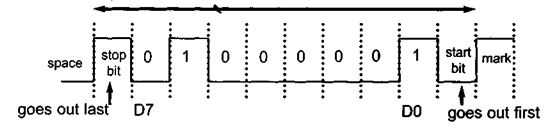
\includegraphics[scale=0.4]{example}
			\item<+-|alert@+> Notice that the LSB is sent out first.
	\end{itemize}
\end{frame}

 \begin{frame}
 	\hskip4cm
 	\textbf{\LARGE Thank You!} \\[20pt]
 	\hskip3cm
 	\scriptsize Post your queries on: 
 	\hyperref[www.e-yantra.org]{\color{blue} http://qa.e-yantra.org/ \color{black}} 
 \end{frame}
\end{document}